\documentclass[thesis.tex]{subfiles}

\begin{document}
\ifSubfilesClassLoaded{
  \setcounter{chapter}{3}
}

\chapter{Estimating duration using biomarkers} \label{ATACCC}

\Cref{E-inc-prev} showed that the duration of RT-PCR positivity is a key parameter for estimating the incidence of SARS-CoV-2 infections.
The aim of this chapter is to estimate the duration of RT-PCR positivity using the viral load data from the ATACCC study (introduced in \cref{E-biology-data:sec:ataccc}).
I model this biomarker over the course of an infection.
From this model, I derive the distribution of the duration of RT-PCR positivity.

First, I will explain how biomarkers are typically modelled, both for SARS-CoV-2 and historically in the biostatistical literature (\cref{ATACCC:sec:background}).
Next, I describe the model of \textcite{hakkiOnset} in detail, which applies these methods to the ATACCC data (\cref{ATACCC:sec:hakki}), before modifying its observation model to improve the robustness of the inference (\cref{ATACCC:sec:observation-modification}).
This modification is based on an earlier analysis using a preliminary version of the dataset, described in \cref{ATACCC:sec:original-analysis}.
I convert the model and parameter estimates of the biomarker's trajectory to a duration of RT-PCR positivity (\cref{ATACCC:sec:duration}).
Finally, I discuss the results (\cref{ATACCC:sec:discussion}).

\section{Background} \label{ATACCC:sec:background}

Two major approaches have been taken to model SARS-CoV-2 viral load trajectories, both based on well-established methods within biostatistics.
The first approach is an ODE-based approach that uses parameters representing biological properties of the virus and host~\autocite[e.g.][]{ejimaEstimation,keVivo,kimQuantitative,goncalvesTiming,perelsonMechanistic}.
The model here is an application of a standard model for viral dynamics, used for many diseases~\autocite{perelsonMechanistic,hernandez-vargasInhost}.
Such models are rarely analytically tractable and the system's evolution is computed using numerical methods.
% Both of these approaches have been used with other viruses and biomarkers.
The second approach, and the focus of this chapter, is using a piecewise linear model for the biomarker trajectory and random effects to allow for within-individual correlation.

Piecewise linear, random effect models have a long history of use for longitudinal data in biostatistics (reviewed by \textcite{slateStatistical}).
Often, as here, they are used to model the temporal evolution of biomarkers.
A few example applications are: CD4 counts following HIV infection~\autocite{langeHierarchical,lynchPredicting} and parasite density in blood samples following malaria treatment~\autocite{fogartyBayesian}.

In these models, the function's parameters are clearly related to features of the biomarker's trajectory, such as the time from first detection to peak viral load, and the viral load at the peak.
The piecewise linear model is the most common in the context of SARS-CoV-2 viral load~\autocite[e.g.][]{clearyUsing,kisslerViral,larremoreTest}
In this context, the piecewise linear model is applied to the log of the viral load.
Hence, the log of the viral load increases linearly, peaks instantaneously, and then decreases linearly; more flexible functions have also been suggested~\autocite{quiltyQuarantine}.

The model for the trajectory I adopt in this chapter, from \textcite{hakkiOnset}, is based on the piecewise log-linear model.
However, they approximate the model so that the function is continuous (see \cref{ATACCC:sec:hakki} for details).

Random effects represent the within-individual correlation while borrowing information between individuals~\autocite[chapter 24]{lashModern}.
Measurements of viral load from the same individual are correlated.
A random effect means that these measurements share parameter(s), providing correlation.
However, the random effect(s) for each individual is drawn towards a common mean, allowing information on their value to be shared between individuals.
Bayesians often refer to random effect models as hierarchical or multilevel models because they can be interpreted as placing a prior at two levels of a parameter hierarchy~\autocite[chapter 5]{gelmanBDA}.
% $\phi_j$ would be referred to as the bottom level of the hierarchy, with $\mu$ and $\sigma$ being the top level.
% More complex models could have more levels, for instance if the individuals are grouped into subpopulations.

% Random effects are used to capture the variation between individuals and the correlation between measurements within the same individual.
% In this context, a random effect means that parameter values are specific to each individual, rather than being a population average.
% The parameter's distribution across the population is assumed to be some known distribution, normally a normal or log-normal distribution~\autocite[chapter 24]{lashModern}.
% Specifically, if $\phi_j$ is the value of some parameter for individual $j$, $\mu_\phi$ is the population mean of $\phi$, and $\sigma_\phi$ is the population standard deviation, then we model $\phi_j$ as: $\phi_j \sim \N(\mu_\phi, \sigma_\phi^2)$ or $\phi_j \sim \LN(\mu_\phi, \sigma_\phi^2)$.
% $\mu_\phi$ and $\sigma_\phi$ are parameters; in a Bayesian setting, a prior is placed on them in the normal way.
% This generalises to a vector of parameters per individual, $\vec{\phi}_j$, in the obvious way.
% In this chapter, $\mu_\phi$ and $\sigma_\phi$ are the parameters of interest, because we want to generalise our model across the population.
% The $\phi_j$s, which tells us about the parameter only for individuals in our sample, are considered nuisance parameters.

\section{\texorpdfstring{\textcite{hakkiOnset}}{Hakki et al. (2022)}} \label{ATACCC:sec:hakki}

The model of \textcite{hakkiOnset} has two components: a latent viral load model and an observation model.
The viral load model is a deterministic function of the model parameters, producing an individual's viral load trajectory.
The observation model mathematically formalises how the RT-PCR testing process produces noisy observations of the latent viral load.
The observation model includes the possibility of false positive and negatives, and the limit of detection of the RT-PCR test (\cref{E-biology-data:sec:PCR}).
% The limit of detection means that viral loads below a certain threshold are not detected by the RT-PCR test.
% They can be represented as a censoring of the viral load at the limit of detection.

Several features of the \textcite{hakkiOnset} model can be motivated by the desire to apply Stan, a modern and convenient implementation of the NUTS (the No U-Turn Sampler) algorithm (see \cref{E-MCMC}).
The first of these is using a continuous viral load trajectory rather than the more common piecewise linear model.
As NUTS uses gradient information, it is more efficient when the model is differentiable.
This leads to the following model for the viral load (see \cref{ATACCC:fig:viral-load-model}):
\begin{align}
v_i(t) = v_{\max,i} \frac{a_i+b_i}{b_ie^{-a_i(t-\tau_{\max,i})} + a_ie^{b_i(t-\tau_{\max,i})}}. \label{ATACCC:eq:viral-load}
\end{align}
Time, $t$, is continuous and defined for individual $i$ such that $i$s first test is at $t = 0$.
$v_{\max,i}$ is the maximum viral load, which occurs at time $\tau_{\max,i}$.
As $\lvert t - \tau_{\max} \rvert$ becomes large, the viral load trajectory tends towards exponential growth (before the peak) or decline (after the peak) in viral load at rates $a_i$ and $b_i$ respectively.
% Before the peak, this is because $b(t-\tau_{\max,i})$ is small and hence $a\exp(b(t-\tau_{\max,i}))$ is negligible.
% After the peak, this is because $b\exp(-a(t-\tau_{\max,i}))$ is negligible.
This happens quickly for realistic values of the parameters.
Therefore, the log viral load is approximately piecewise linear (see \cref{ATACCC:fig:viral-load-model} for representative viral load trajectories).
$\vec{\phi}_i = (v_{\max,i}, a_i, b_i)^T$ are the random effects for individual $i$.

$\tau_{\max,i}$ is a fixed effect for each individual because time is defined for each individual based on when they are first tested.
This time is based on logistical and behavioural factors such as delays in the NHS Test and Trace system and the study design.
\begin{figure}[tbhp]
  \centering 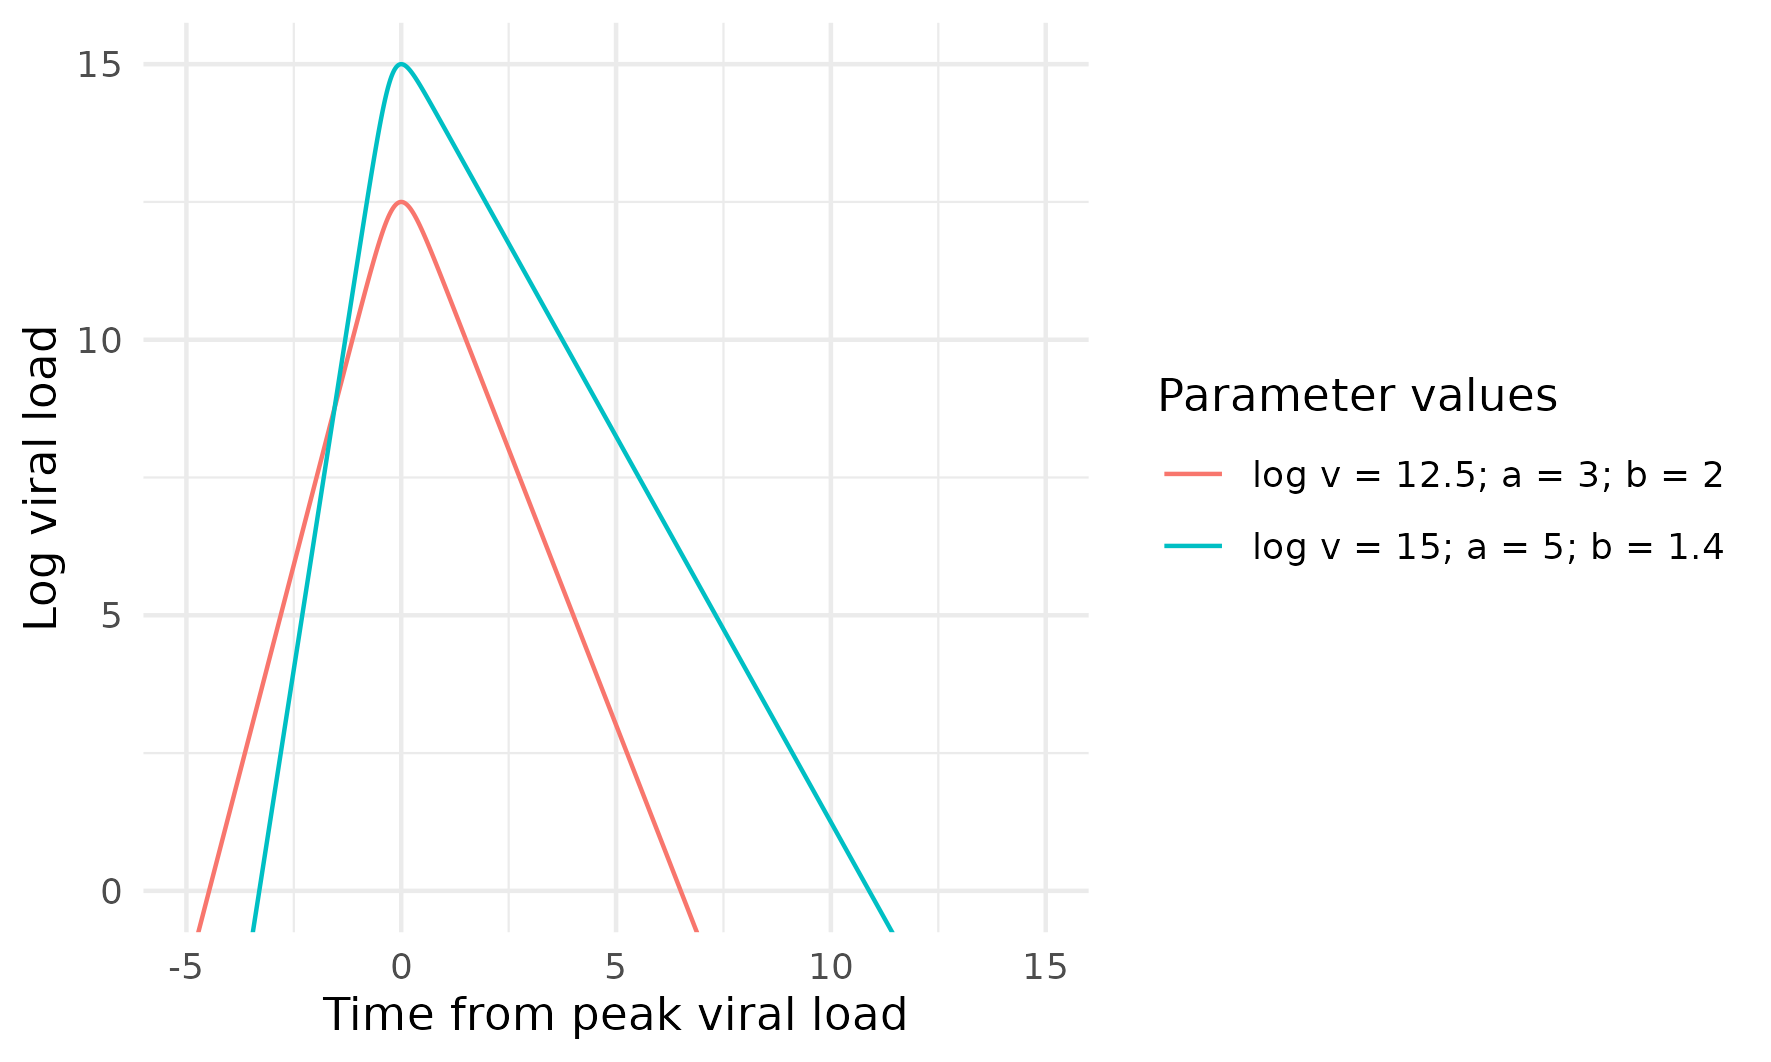
\includegraphics{ATACCC/typical_trajectory}
  \caption[Example viral load model trajectory.]{%
    Example viral load trajectory produced by \textcite{hakkiOnset}'s viral load model, using realistic parameter values.
    The increase and decrease in log viral load are approximately linear with a gradient of $a_i$ and $b_i$ respectively.
    The peak is at time $\tau_{\max,i} = 0$ and log viral load $\log v_{\max,i}$.
    The key omits subscripts for brevity.
  }
  \label{ATACCC:fig:viral-load-model}
\end{figure}

The noise in the RT-PCR test result is modelled by assuming each measurement of log viral load has an iid error distributed $\N(0, \sigma_v^2)$.
Measurements are left censored at the limit of detection, $\vlod$, meaning that any observation which would give a log viral load of less than $\vlod$ is instead observed as negative.
False positives and negatives are modelled by allowing a test failure with probability $\rho$.
Test failures are modelled as producing a log viral load reading drawn from $\N(x_0, \sigma_0^2)$.
These readings are censored in the same way as true readings.
A censored test failure represents a false negative, otherwise the test failure represents a false positive.
\textcite{hakkiOnset} uses a prior for $x_0$ centred on $\vlod$, which encodes a prior belief that false negatives and false positives occur with equal probability.

Let the observed log viral load for individual $i$ at time $t$ be $y_{i,t}$, with negative tests signified by $y_{i,t}=v_\text{lod}$.
Then, the likelihood contribution of this observation is:
\begin{align}
p(y_{i,t} \mid \cdot) &= \begin{cases}
    \rho f_N(y_{i,t} \mid x_0, \sigma_0^2) + (1 - \rho) f_N(y_{i,t} \mid \log v_i(t), \sigma_v^2) & \text{if $y_{i,t} > v_\text{lod}$}\\
    \rho F_N(v_\text{lod} \mid x_0, \sigma_0^2) + (1 - \rho) F_N(\vlod \mid \log v_i(t), \sigma_v^2) & \text{if $y_{i,t} = v_\text{lod}$} \label{ATACCC:eq:hakki-likelihood}
\end{cases}
\end{align}
where $f_N(y \mid \mu, \sigma^2)$ and $F_N(y \mid \mu, \sigma^2)$ are the pdf and cdf at $y$ of a normal distribution with mean $\mu$ and variance $\sigma^2$ respectively.
The first term on each line is the likelihood contribution from test failures, either a false positive (top line) or false negative (bottom line).
The second term is the likelihood contribution from non-failed test results, either measurements of viral load (top line) or negative results (bottom line).

Conditional on all parameters, the observations are assumed independent.
Because $v_i$ is a deterministic transform of $\vec{\phi}_i$ and $\tau_{\max,i}$, the observations are independent conditional on the model parameters, and the full likelihood is the product of the likelihoods of each observation.

Individuals are split into groups based on their vaccination status.
The first group is unvaccinated and infected with a variety of pre-Alpha, Alpha, and Delta variants.
The second group is vaccinated, and all were infected by the Delta variant.
My focus is on the first group since they most closely correspond to the infections in the time period used throughout this thesis.

Biological plausibility requires constraining $\vec{\phi}_i$ to positive real values.
Each $\vec{\phi}_i$ is modelled as a log-normal random effects by using the hierarchical prior $\vec{\phi}_i \dist \LN(\vec{\mu}_{\phi,g(i)}, \matr{\Sigma}_\phi)$ where $g(i)$ is the group of individual $i$.
$\vec{\mu}_{\phi,g} = [\mu_{v_{\max},g}, \mu_{a,g}, \mu_{b,g}]^T$ is a vector of the population means of the log-parameters.
As the random effects have a log-normal, rather than normal, distribution $\exp(\vec{\mu}_{\phi,g})$ is the population median of the parameter value but not the mean.
The covariance matrix $\matr{\Sigma}_\phi$ controls the variability of the population and allows for the parameters to be correlated.
For example, an individual with a high peak viral load may also clear the virus slowly because both have an underlying cause of a weak immune system.
To improve sampling efficiency, the multivariate version of the non-centred parameterization~\autocite{papaspiliopoulosGeneral,stanReparameterization} is used.
This can be expressed as follows.
\begin{align}
  \vec{\eta}_i &\dist \N(\vec{0}, \matr{C}_\phi) \\
  \log \vec{\phi}_i &= \vec{\mu}_{\phi,g(i)} + \vec{\sigma}_\phi \circ \vec{\eta}_i
\end{align}
where $\vec{\sigma}_\phi$ is a vector of the standard deviations of the parameters, and $\matr{C}_\phi$ is a correlation matrix.
These are defined such that, by construction, $(\matr{\Sigma}_\phi)_{ij} = (\vec{\sigma}_\phi)_i (\vec{\sigma}_\phi)_j (\matr{C}_\phi)_{ij}$.
% Correlation matrices have diagonal elements all 1, therefore this reparameterization has the same number of parameters as the original model.

\textcite{hakkiOnset} uses weakly informative priors, similar to \textcite{singanayagamCommunity}, see \cref{ATACCC:table:hakki-priors}.
I reran \textcite{hakkiOnset}'s analysis using R~4.3.1~\autocite{R-4-3-1}.
The inference was performed using RStan~2.32.3~\autocite{RStan-2-32-3} and Stan~2.32.2~\autocite{Stan-2-32-2}.
Inference settings were the same as \textcite{hakkiOnset}, which included 8 chains with a total of \numprint{8000} iterations each with the first \numprint{3000} used as warm-up.
\begin{table}
\begin{tabular}{l c l l}
    Parameter description & Symbol & Distribution \\
    \hline \\
    Mean max log viral load & $\mu_{v_\text{max}, g}$ & $\N(15, 15^2)$ \\
    Standard deviation of max log viral load & $\sigma_{v_\text{max}}$ & $\N_+(0, 10^2)$ \\
    Mean rate of log viral load increase & $\mu_{a, g}$ & $\N(1.25, 0.75^2)$ \\
    Standard deviation of rate of log viral load increase & $\sigma_{a}$ & $\N_+(0, 1)$ \\
    Mean rate of log viral load decrease & $\mu_{b, g}$ & $\N(0.5, 1.4^2)$ \\
    Standard deviation of rate of log viral load decrease & $\sigma_{b}$ & $\N_+(0, 1)$ \\
    Correlation of viral load parameters & $\matr{C}_\phi$ & $\LKJ(1)$ \\
    Negative log of rate of test failure & $-\log \rho$ & $\N(3, 0.5)$ \\
    Mean log viral load for test failures & $x_0$ & $\N(0, 3^2)$ \\
    Standard deviation of log viral load for test failures & $\sigma_0$ & $\N_+(3, 3^2)$ \\
    Standard deviation of log viral load observations & $\sigma_v$ & $1 + \N_+(2, 3^2)$ \\
    Time from first test to peak & $\tau_{\max,i}$ & $\N(5,5)$
\end{tabular}
\caption[Viral load model priors]{Priors for each parameter, taken from \textcite{hakkiOnset}. $\N_+$ indicates a normal distribution truncated to the non-negative reals. Details of all distributions used, including their parameterizations, are in \cref{E-distributions}. The elements of $\vec{\mu}_{\phi,g}$ and $\vec{\sigma}_\phi$ have independent priors placed on them, as specified in the first lines of the table. Priors are the same for all $g$ and $i$. \label{ATACCC:table:hakki-priors}}
\end{table}

\section{Modifying the Hakki observation model} \label{ATACCC:sec:observation-modification}

The model of \textcite{hakkiOnset} did not converge fully (see \cref{ATACCC:sec:results}).
In particular, the Rhat values, traceplots, and effective sample size for the parameters of the observation model ($x_0$, $\sigma_0$, and $\rho$) were poor.

Based on the fit to the data achieved when implementing an earlier version of the model (see \cref{ATACCC:sec:original-analysis}), I hypothesised that the cause of this was overcomplicating the model for test failures.
Specifically, excluding false positives from the model still explains the data well (see \cref{ATACCC:fig:goodness-of-fits}).
Furthermore, a prior that false negatives and false positives are equally likely is not supported by other information (see \cref{E-biology-data:sec:measurement-error}).
Therefore, I simplified the model for test failures to only false negatives.
% These false negatives could represent a variety of scenarios, such as poor swabbing technique.
Formally, I replaced \cref{ATACCC:eq:hakki-likelihood} with the following.
\begin{align}
p(y_{i,t} \mid \cdot) &= \begin{cases}
    (1 - \rho) f_N(y_{i,t} \mid \log v_i(t), \sigma_v^2) & \text{if $y_{i,t} > v_\text{lod}$}\\
    \rho + (1 - \rho) F_N(\vlod \mid \log v_i(t), \sigma_v^2) & \text{if $y_{i,t} = v_\text{lod}$.}
\end{cases}
\end{align}

The parameters $x_0$ and $\sigma_0$ are no longer used in the model.

I reanalyse the data using this modified model.
The priors are the same as \textcite{hakkiOnset}, including the prior on $\rho$, and performed inference with the same settings (described at the end of \cref{ATACCC:sec:hakki}).


\section{Deriving duration from the parameters} \label{ATACCC:sec:duration}

The ultimate aim of this chapter is to produce an estimate of the distribution for the duration of RT-PCR positivity.
So far, only the viral load trajectories have been considered; \textcite{hakkiOnset} does not consider duration.
In this section, I derive an expression for individual $i$'s infection episode duration, $d_i$, in terms of $\vec{\phi}_i$.

The time that individual $i$ is first and last detectable are the two values of $t$ such that $\log v_i(t) = v_\text{lod}$.
Denote these times as $\tau_{0,i}$ and $\tau_{1,i}$.
Hence, $d_i = \tau_{1,i} - \tau_{0,i}$.

At $\tau_{0,i}$ and $\tau_{1,i}$, the approximation as exponential growth (described in \cref{ATACCC:sec:hakki}) is good, meaning that one of the exponential terms in the denominator of \cref{ATACCC:eq:viral-load} is 0.
Substituting in this, and $\log v_i(\tau_{0,i}) = \log v_i(\tau_{1,i}) = v_\text{lod} = 0$, gives the following expressions for $\tau_{0,i}$ and $\tau_{1,i}$.
\begin{align}
\tau_{0,i}
&= \tau_{\max,i} - \frac{1}{a_i} \left(\log v_{\max,i} + \log(a_i + b_i) - \log b_i \right) \\
\tau_{1,i}
&= \tau_{\max,i} + \frac{1}{b_i} \left(\log v_{\max,i} + \log(a_i + b_i) - \log a_i \right) \\
d_i
&= \tau_{1,i} - \tau_{0,i}  \\
&= \frac{1}{a_i b_i} \left( (a_i + b_i) (\log v_{\max,i} + \log(a_i + b_i)) - a_i \log a_i - b_i \log b_i \right).
\label{ATACCC:eq:di}
\end{align}

From \cref{ATACCC:eq:di}, we can see that $d_i$ depends only on $i$'s random effects vector $\vec{\phi}_i$.
Therefore, the distribution of $d_i$ across the population of group $g$ is determined by $\vec{\phi}_i$'s mean, $\vec{\mu}_{\phi,g}$, and covariance matrix, $\matr{\Sigma}_\phi$.
% Hence, the uncertainty in the posterior distribution of the discretised duration cumulative distribution function for group $g$, $F_{D,g}(d) = \prob(D_i \leq d + 0.5)$ originate from the uncertainty in $\vec{\mu}_\phi$ and $\matr{\Sigma}_\phi$.

For a known $\vec{\mu}_{\phi,g}$ and $\matr{\Sigma}_\phi$, $F_{D,g}$ is found as:
\begin{align}
  F_{D,g}(d)
  &= \prob(D_i \leq d + 0.5) \\
  &= \E_{D_i}(\I(D_i \leq d + 0.5))
  \label{ATACCC:eq:FDintegral}
\end{align}
where $\I$ is the indicator function.
The integral in \cref{ATACCC:eq:FDintegral} can be approximated using Monte Carlo integration (see \cref{ATACCC:alg:MonteCarlo}).
Equivalent forms of $F_{D,g}$, such as the survival and hazard functions, can be calculated using the relations in \cref{E-inc-prev:sec:definitions}.

\begin{algorithm}
\For{$i = 1, \dots, N$}{
  \For{$j = 1, \dots, M$}{
    Sample an individual-level random effects vector $\vec{\phi}_{i,j} \dist \LN(\vec{\mu}_{\phi,g}^{(i)}, \matr{\Sigma}^{(i)}_\phi)$ \;
    Calculate $d_{i,j}$ using \cref{ATACCC:eq:di} \;
  }
  \For{$d = 1, \dots, \dmax$}{
    Set $F_{D,g}^{(i)}(d) = \frac{1}{M} \sum_{j=1}^M \I(d_{i,j} \leq d + 0.5)$ \;
  }
}
  \caption{%
  Algorithm to calculate the Monte Carlo integral in \cref{ATACCC:eq:FDintegral}, producing the posterior distribution of $F_{D,g}(d)$.
  The posterior distribution is represented as a sample $F_{D,g}^{(1)}, \dots, F_{D,g}^{(N)}$.
  $\vec{\mu}_{\phi,g}^{(i)}$ and $\matr{\Sigma}_\phi^{(i)}$ denote the $i$th posterior sample of $\vec{\mu}_{\phi,g}$ and $\matr{\Sigma}_\phi$ respectively, taken from the MCMC output which produced $N$ posterior samples.
  $M$ is the number of individuals to draw, I found $M =\numprint{100000}$ produced stable estimates of the tail of $F_{D,g}(d)$ if $\dmax = 45$.
 }
 \label{ATACCC:alg:MonteCarlo}
\end{algorithm}

Applying \cref{ATACCC:alg:MonteCarlo} produces a sample of the posterior distribution of $F_{D,g}(d)$.
One sample is produced for each iteration of the MCMC (Markov Chain Monte Carlo) output used to estimate $\vec{\mu}_{\phi,g}$ and $\matr{\Sigma}_\phi$.

\section{Results} \label{ATACCC:sec:results}


The original \textcite{hakkiOnset} model has convergence issues (Rhat > 1.07 and ESS (Effective Sample Size) < 100) for the parameters of the test failure distribution, $\sigma_0$ and $\rho$.
The simplified model I proposed in \cref{ATACCC:sec:observation-modification} solved this issue, meaning that this analysis converged.

The two models give very similar estimates for the population-level parameters (see \cref{ATACCC:fig:compare-hakki-modified}).
These are the main parameters of interest (as explained in \cref{ATACCC:sec:duration}), suggesting that the results are robust to the choice of model.
As the estimates are similar and the modified model converges better, I will use only the results from the modified model.
In this study, $\vlod = 0$.
\begin{figure}
  \centering 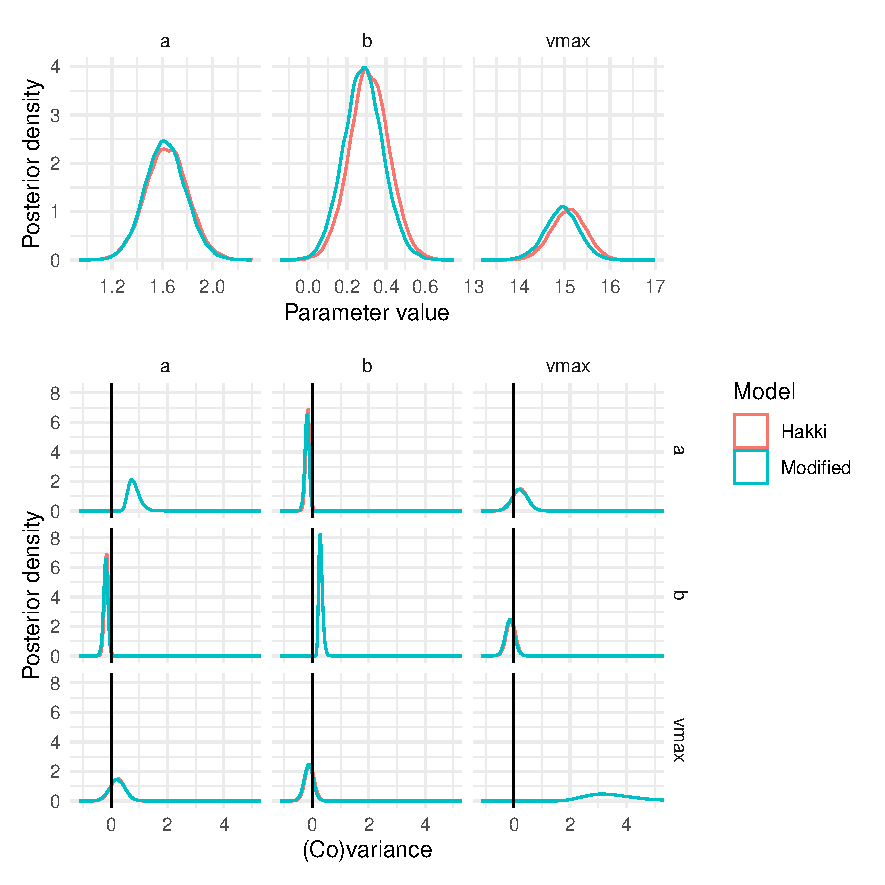
\includegraphics{ATACCC/compare_hakki_modified}
  \caption[Comparison of population-level parameters between models.]{Kernel-density smoothed posterior densities for the population mean (top), $\vec{\mu}_{\phi,1}$, and covariance matrix (bottom), $\matr{\Sigma}_\phi$, for both the \textcite{hakkiOnset} model (described in \cref{ATACCC:sec:hakki}) and the model with a modified observation model to improve convergence (described in \cref{ATACCC:sec:observation-modification}). Mean only shown for the unvaccinated group, the primary group of interest. The groups share the covariance matrix. These parameters, which are the primary ones of interest (see \cref{ATACCC:sec:duration}), have very similar estimates between the models. \label{ATACCC:fig:compare-hakki-modified}}
\end{figure}

Clear differences emerge between the vaccinated and unvaccinated groups (see \cref{ATACCC:fig:median-trajectories} and \cref{ATACCC:table:population-estimates}).
The rates of viral load increase at similar rates in the two groups, the vaccinated group have higher peak viral loads and clear the virus faster.
This leads to a shorter duration of RT-PCR positivity in the vaccinated group.
\begin{figure}
  \centering 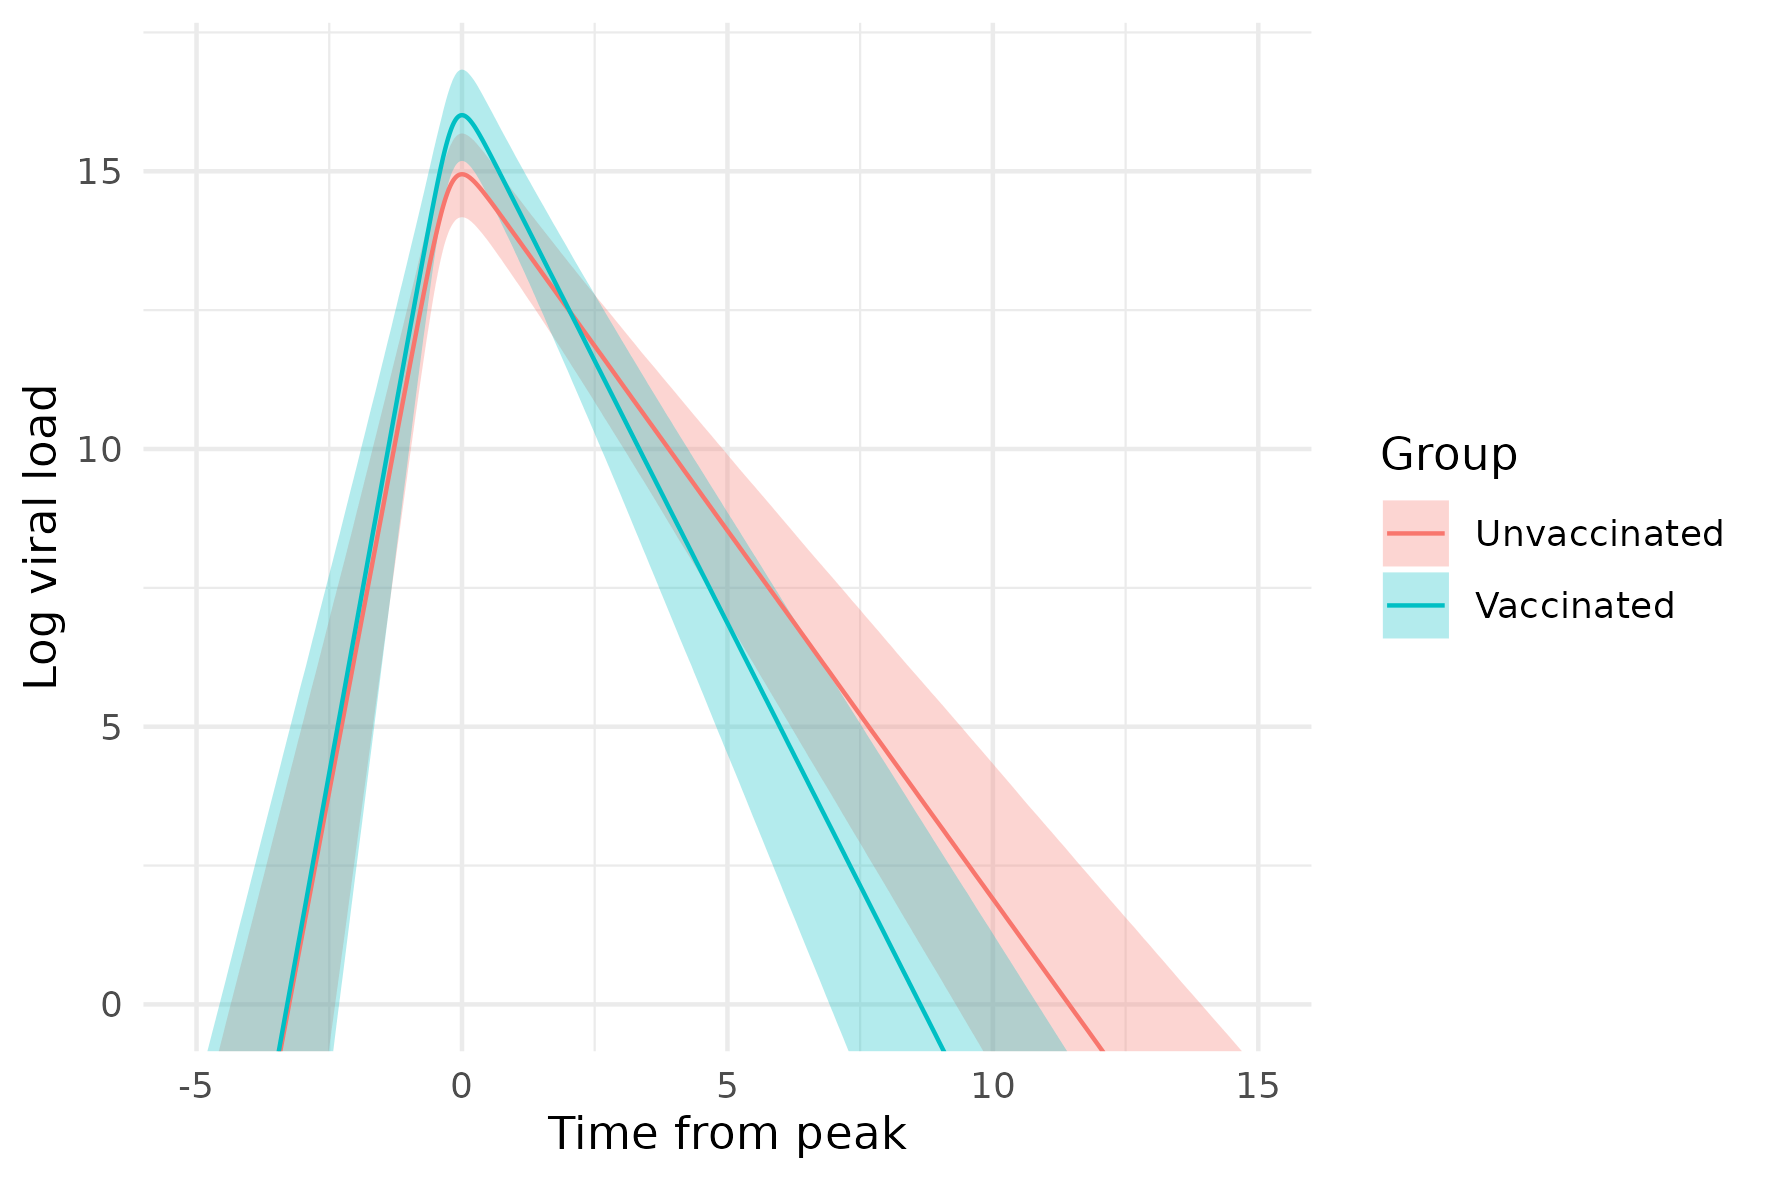
\includegraphics{ATACCC/mean_trajectories}
  \caption[Median viral load trajectories]{Trajectory (posterior median and 95\% CrI) using the population median parameter values, $\exp \vec{\mu}_{\phi,g}$, excluding the within-population variation. These assume $\tau_{\max,i}=0$, however modifying this simply translates the trajectories left or right. \label{ATACCC:fig:median-trajectories}}
\end{figure}
\begin{table}
  \makebox[\linewidth]{
  \begin{tabular}{lcc}
    Parameter & Unvaccinated population & Vaccinated population \\
    Max log viral load, $\mu_{v_\text{max},g}$ & 14.9 (14.2--15.7) & 16.0 (15.2--16.8) \\
    Rate of log viral load increase, $\exp(\mu_{a,g})$ & 5.07 (3.70--7.06) & 1.25 (1.18--1.32) \\
    Rate of log viral load decrease, $\exp(\mu_{b,g})$ & 1.33 (1.09--1.63) & 1.89 (1.50--2.36) \\
  \end{tabular}
  }
  \caption{Population-level estimates of the viral load parameters (posterior medians and 95\% CrI). The vaccinated population have higher peak viral loads but clear the virus faster. \label{ATACCC:table:population-estimates}}
\end{table}

The false negative rate, $\rho$, is estimated to be quite low, 5.3\% (95\% CrI: 3.7--7.3\%).
The test sensitivity, which will be relevant in \cref{E-imperf-test}, is the probability that a detectable individual tests positive, $\psens = 1 - \rho$.

The $F_{D,g}$ estimates for the two groups are in \cref{ATACCC:fig:duration}.
The vaccinated population very likely has a shorter duration of RT-PCR positive (93\% posterior probability of a shorter median duration) than the unvaccinated population (see \cref{ATACCC:fig:duration}).
The median duration of RT-PCR positivity for the vaccinated population is 13 days (95\% CrI: 11--16 days), but it is 16 days (95\% CrI: 14--19 days) for the unvaccinated population.
\begin{figure}
  \centering 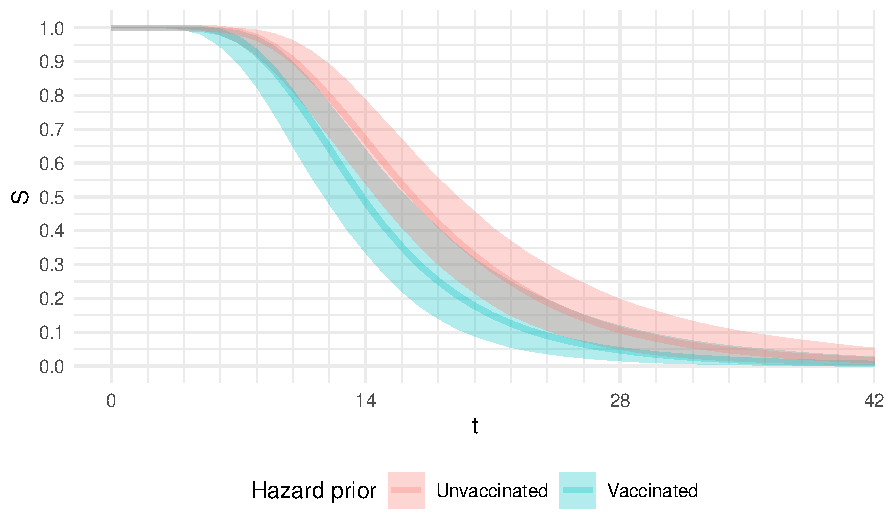
\includegraphics{ATACCC/duration}
  \caption[Duration of RT-PCR positivity.]{Estimated distribution (survival function) of duration of RT-PCR positivity for the two populations. The vaccinated population have shorter durations of RT-PCR positivity.  \label{ATACCC:fig:duration}}
\end{figure}

The modified model produced good fits to the data (see \cref{ATACCC:fig:goodness-of-fits,ATACCC:fig:appendix-goodness-of-fits}).
Almost all test results are captured in the 95\% credible intervals.
\begin{figure}
  \makebox[\textwidth][c]{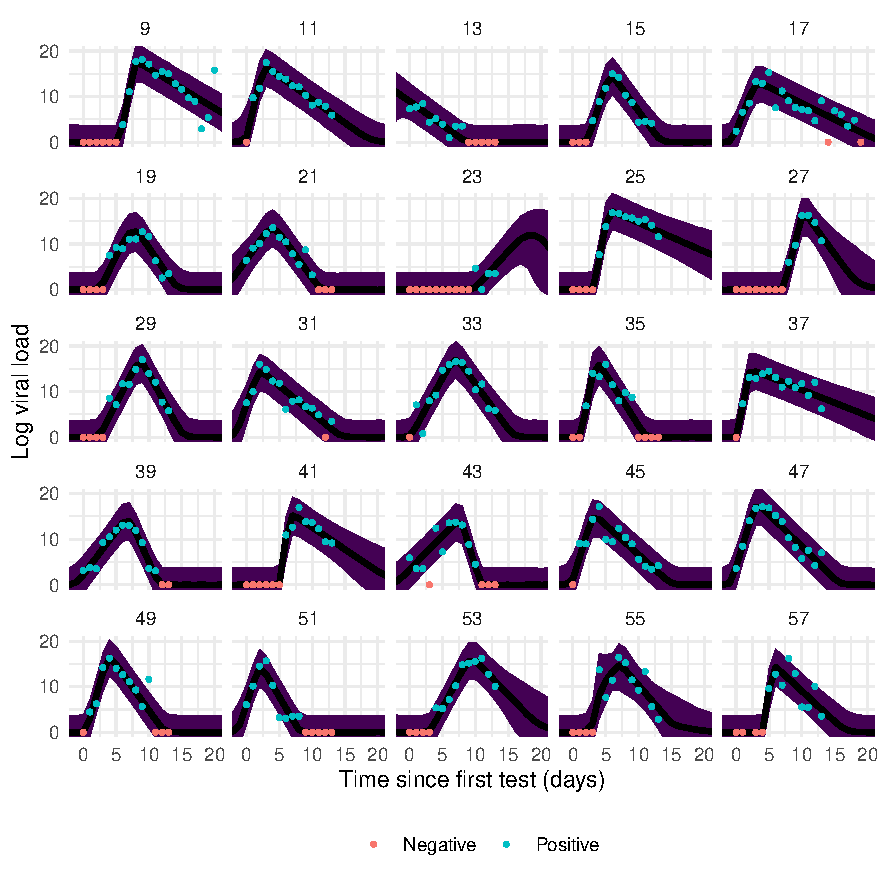
\includegraphics[width=.9\paperwidth]{ATACCC/fits}}
  \caption[Posterior predictive viral load fits]{Posterior predictive observed viral loads (median and 95\% CrI, lines and ribbon) for selected individuals, overlaid with their observed test results (dots). Posterior estimates are conditional on the result not being a false negative. Negative RT-PCR tests are plotted at the limit of detection, \ie a log viral load of 0. Each plot is labelled with the individual's position in the dataset, an arbitrary value.
  Remaining individuals shown in \cref{ATACCC:fig:appendix-goodness-of-fits}.
  \label{ATACCC:fig:goodness-of-fits}}
\end{figure}

For individual-level parameters, both models had convergence issues in places (Rhat > 1.4 and ESS < 20).
However, this was greatly improved with the simplified model, occurring only for parameters relating to a single individual, number 55.

Individual 55 has an extremely noisy set of observations (see \cref{ATACCC:fig:goodness-of-fits}).
This means that two viral load trajectories fit the data well (shown in \cref{ATACCC:fig:individual-55}).
The first, found by two chains, increases very quickly, peaks 4.0 days after the first test, then declines slowly.
The second, found by the other six chains, is more symmetrical, peaking 7.2 days after the first test.
The population-level parameter estimates agree between the two sets of chains (not shown); therefore, the issue should not affect any estimates of interest.
\begin{figure}
  \centering 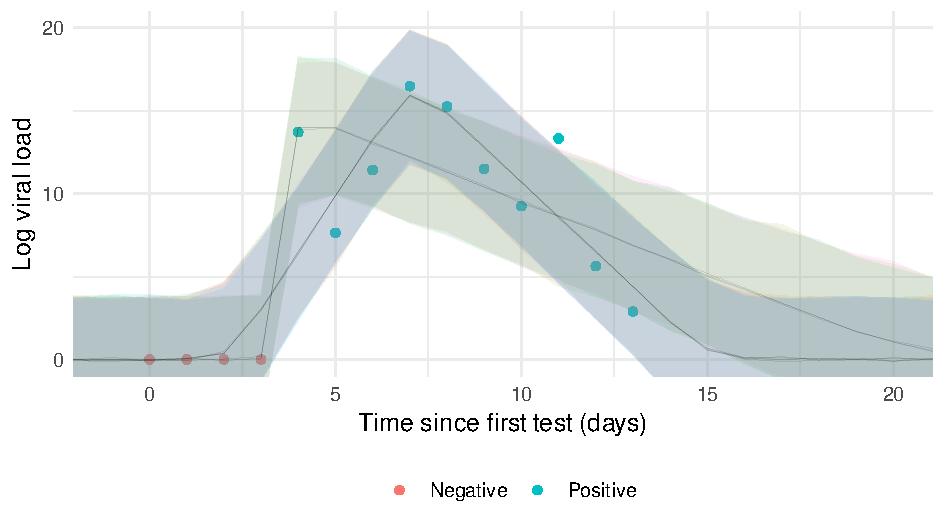
\includegraphics{ATACCC/fit_individual_55}
  \caption[Goodness-of-fit for individual 55]{Fit to individual 55's data coloured by MCMC chain. Two chains favour the quickly increasing viral load trajectory, peaking at day 4.0, the other six favour the slower trajectory, peaking at day 7.2. \label{ATACCC:fig:individual-55}}
\end{figure}

\section{Discussion} \label{ATACCC:sec:discussion}

Different estimates were produced for vaccinated and unvaccinated individuals in the study.
However, there are many differences between individuals in these two groups.
For example, the vaccinated individuals are likely to be older and/or have co-morbidities because the roll-out of the vaccine in the UK prioritised these groups~\autocite{naoCovidVaccination}.
They were also infected by different variants because the infections in vaccinated individuals occurred later.
All these factors could change the viral dynamics~\autocite{russellWithinhost,kisslerDynamicsVaccines} and hence the duration.
Therefore, the relationships shown here are not causal, or even generalisable to contexts where these other confounders are not present.
Despite these confounders, the result is in agreement with previous work showing that the Alpha and Delta variants of concern (compared to pre-Alpha variants) and being vaccinated are all associated with shorter durations of RT-PCR positivity, although the vaccination effect is larger~\autocite{kisslerDynamicsVaccines}.

A strength of the ATACCC data are its general population sample.
This is unlike most estimates (see \cref{E-intro:sec:previous-duration-estimates}) which are from hospitalised patients or healthcare workers.
This means that, notwithstanding the issues highlighted in the previous paragraph, the estimates are likely to be generalisable to the general population.

Individuals 55 and 57 appear to have far noisier measurements than the other individuals (see \cref{ATACCC:fig:goodness-of-fits}), suggesting that the observation noise might vary between individuals.
Including a random effect on $\sigma_v$ could capture this affect.
However, it would complicate the model, be unlikely to change the estimates of the parameters of interest and may not be identifiable.

In the ATACCC study, individuals were tested for at most 20 days.
Yet, the estimates here still have 33\% (95\% CrI: 21--46\%) of individuals positive at 20 days following infection.
The remainder of the estimate for $f_D$, such as that almost all (>99\%) of individuals recover before day 50, is driven by the assumed form of the viral load trajectory.

\section{Conclusion}

This chapter has estimated the distribution of RT-PCR positive duration based on the viral load data from the ATACCC study.
In the following chapters, I will use the estimates from the unvaccinated individuals.
The CIS data I use is from autumn 2020 and early 2021 when few individuals were vaccinated, and the majority of infections were by pre-Alpha or Alpha variants.
Therefore, this group of people should be fairly representative of those within CIS.

A major issue with the estimates of duration presented here is that the number of individuals who test positive for a long period of time is based on extrapolation of the viral load model.
In periods of low incidence following a large peak, prevalent individuals could be mostly infected a long time ago.
Therefore, understanding if these probabilities are correct is important for understanding transmission in the period after a peak.
These effects are even more prominent when incidence falls suddenly to low levels due to an intervention such as a lockdown.
This is exactly the situation in the UK in early 2021.
The next two chapters will incorporate CIS data to improve the estimates of these tail probabilities.
Therefore, I will now incorporate the CIS data to improve the estimates of the tail probabilities of the duration of RT-PCR positivity.

\ifSubfilesClassLoaded{
  \appendix
  \subfile{distributions}
  \subfile{ATACCC-appendix-original-analysis}
  \listoftodos
}{}

\end{document}